
%%%%%%%%%%

%\begin{figure}[h]

\centering
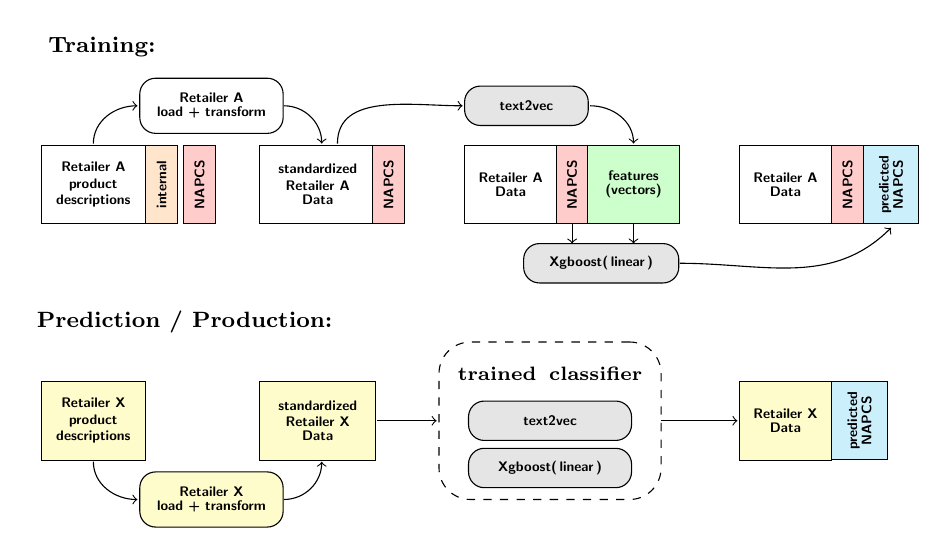
\begin{tikzpicture}
[node distance = 1cm, auto,font=\scriptsize,
% STYLES
every node/.style={node distance=3cm},
% The comment style is used to describe the characteristics of each force
comment/.style={rectangle, inner sep= 5pt, text width=4cm, node distance=0.25cm, font=\scriptsize\sffamily},
% The force style is used to draw the forces' name
force/.style={rectangle, draw, fill=black!10, inner sep=1pt, text width=1.1cm, text badly centered, minimum height=0.75cm, font=\bfseries\scriptsize\sffamily}] 

%%%  ~~~~~~~~~~  %%%

\node at (0.11,5.75) {\footnotesize\textbf{Training:}};

\node [force, fill=white, minimum height=1.0cm, text width=1.25cm] at (0.0,4) {\tiny Retailer A\vskip 0.0cm product\vskip -0.075cm descriptions};
\node [force, fill=orange!20, minimum height=0.4cm, text width=0.925cm, rotate=90] at (0.865,4) {\tiny internal};
\node [force, fill=red!20, minimum height=0.4cm, text width=0.925cm, rotate=90] at (1.35,4) {\tiny NAPCS};

\draw [->] (0.0,4.52) to [out=90,in=180] (0.56,5.0);
\node [force, fill=white, rounded corners=0.2cm, text width=1.75cm, minimum height=0.7cm] at (1.5,5) {\tiny Retailer A\vskip -0.1cm load + transform};
\draw [->] (2.42,5.0) to [out=0,in=90] (2.9,4.52);

\node [force, minimum height=1.0cm, fill=white, text width=1.4cm] at (2.85,4) {\tiny standardized\vskip 0.0cm Retailer A\vskip -0.1cm Data};
\node [force, minimum height=0.4cm, fill=red!20, text width=0.925cm, rotate=90] at (3.75,4) {\tiny NAPCS};

\draw [->] (3.1,4.52) to [out=90,in=180] (4.69,5.0);
\node [force, fill=gray!20, rounded corners=0.2cm, text width=1.5cm, minimum height=0.5cm] at (5.5,5) {\tiny text2vec};
\draw [->] (6.31,5.0) to [out=0,in=90] (6.86,4.52);

\node [force, minimum height=1.0cm, fill=white] at (5.3,4) {\tiny Retailer A\vskip -0.1cm Data};
\node [force, minimum height=0.4cm, fill=red!20, text width=0.925cm, rotate=90] at (6.08,4) {\tiny NAPCS};
\node [force, minimum height=1.0cm, fill=green!20, text width=1.1cm] at (6.86,4) {\tiny features\vskip -0.1cm(vectors)};

\node [force, fill=gray!20, rounded corners=0.2cm, text width=1.9cm, minimum height=0.5cm] at (6.45,3) {\tiny Xgboost(\,linear\,)};
\draw [->] (6.08,3.5) -- (6.08,3.25);
\draw [->] (6.86,3.5) -- (6.86,3.25);

\node [force, minimum height=1.00cm, fill=white] at (8.79,4) {\tiny Retailer A\vskip -0.1cm Data};
\node [force, minimum height=0.40cm, fill=red!20, text width=0.925cm, rotate=90] at (9.58,4) {\tiny NAPCS};
\node [force, minimum height=0.7cm, fill=cyan!20,   text width=0.925cm, rotate=90] at (10.13,4) {\tiny predicted\vskip -0.1cm NAPCS};
\draw [->] (7.45,3.0) to [out=0,in=225] (10.13,3.45);

%%%  ~~~~~~~~~~  %%%

\node at (1.16,2.25) {\footnotesize\textbf{Prediction / Production:}};

\node [force, fill=yellow!20, minimum height=1.0cm, text width=1.25cm] at (0.0,1) {\tiny Retailer X\vskip 0.0cm product\vskip -0.075cm descriptions};

\draw [->] (0.0,0.48) to [out=270,in=180] (0.56,0.0);
\node [force, fill=yellow!20, rounded corners=0.2cm, text width=1.75cm, minimum height=0.7cm] at (1.5,0) {\tiny Retailer X\vskip -0.1cm load + transform};
\draw [->] (2.42,0.0) to [out=0,in=270] (2.9,0.48);

\node [force, minimum height=1.0cm, fill=yellow!20, text width=1.4cm] at (2.85,1) {\tiny standardized\vskip 0.cm Retailer X\vskip -0.1cm Data};

\node [force, dashed, minimum height=2cm, text width=2.75cm, fill=white, rounded corners=0.4cm] at (5.8,1) {};
\draw [->] (3.6,1) -- (4.36,1);
\draw [->] (7.21,1) -- (8.18,1);
\node at (5.8,1.6) {\scriptsize\textbf{trained\, classifier}};
\node [force, fill=gray!20, rounded corners=0.2cm, text width=2.0cm, minimum height=0.5cm] at (5.8,1) {\tiny text2vec};
\node [force, fill=gray!20, rounded corners=0.2cm, text width=2.0cm, minimum height=0.5cm] at (5.8,0.4) {\tiny Xgboost(\,linear\,)};

\node [force, minimum height=1.00cm, fill=yellow!20] at (8.79,1) {\tiny Retailer X\vskip -0.1cm Data};
\node [force, minimum height=0.7cm, fill=cyan!20,   text width=0.925cm, rotate=90] at (9.73,1) {\tiny predicted\vskip -0.1cm NAPCS};

%%%  ~~~~~~~~~~  %%%

%%%%%%%%

\end{tikzpicture}

%%%%%%%%%%
